\documentclass{beamer}
\usetheme{Warsaw}
\setbeamertemplate{footline}[frame number]

\usepackage[utf8]{inputenc}
\usepackage{fancybox}
\usepackage{multimedia} 
\usepackage{subfig}
\usepackage{amsmath}
\usepackage{hyperref}
\usepackage[all]{xy}
\begin{document}


\title[Angewandte Mathematik] % (optional, only for long titles)
{Angewandte Mathematik
\\
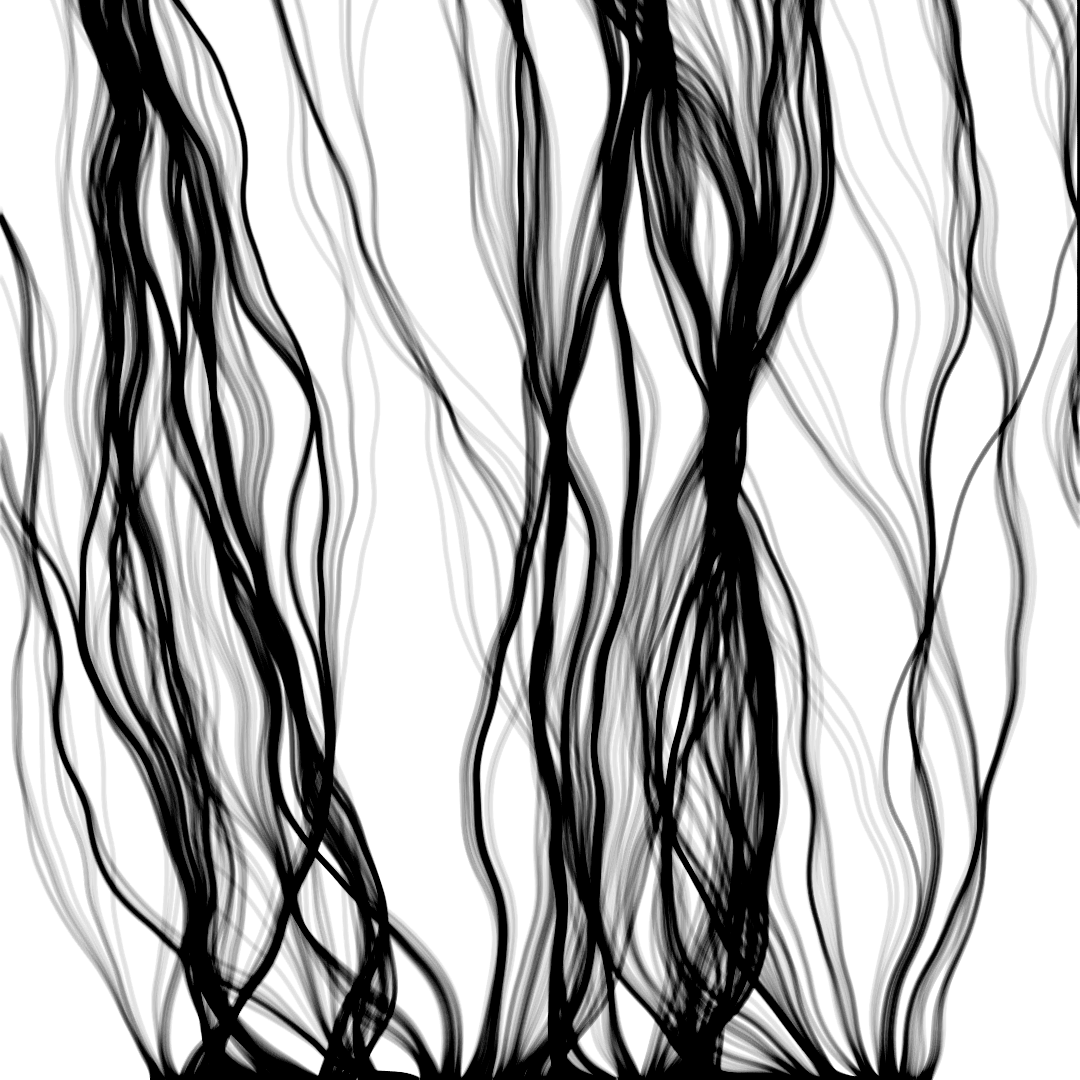
\includegraphics[scale=0.15]{images/cover}
}
\subtitle{}
\author[Dr. Johannes Riesterer] % (optional, for multiple authors)
{Dr.  rer. nat. Johannes Riesterer}

\date[KPT 2004] % (optional)
{}

\subject{Angewandte Mathematik}

\frame{\titlepage}

\begin{frame}
    \frametitle{Angewandte Mathematik}
\framesubtitle{Einleitung Lean}
    \begin{block}{Was ist Lean?}
        \begin{itemize}
            \item Ein interaktiver Theorembeweiser und Programmiersprache.
            \item Wird verwendet, um mathematische Aussagen formal zu beweisen und zu verifizieren.
            \item Besitzt eine aktive und wachsende Community, insbesondere in der formalen Mathematik.
        \end{itemize}
    \end{block}

\begin{block}{Curry Howard Isomorphismus}
   
     Der Curry-Howard-Isomorphismus besagt, dass logische Aussagen als Typen und Beweise als Programme betrachtet werden können. Mit anderen Worten:
    \begin{itemize}
        \item Logische Aussagen $\leftrightarrow$ Typen
    
        \item Beweise von Aussagen $\leftrightarrow$  Programme, die zu diesen Typen gehören
    \end{itemize}
    \end{block}

 \end{frame}


 
 \begin{frame}
    \frametitle{Angewandte Mathematik}
\framesubtitle{Einleitung Lean}
    \begin{block}{Installing Lean}

    \end{block}

\begin{block}{Learning Lean}
    \begin{itemize}
        \item Logische Aussagen $\leftrightarrow$ Typen
    
        \item Beweise von Aussagen $\leftrightarrow$  Programme, die zu diesen Typen gehören
    \end{itemize}
    \end{block}

 \end{frame}




\end{document}

